\documentclass[]{book}
\usepackage{lmodern}
\usepackage{amssymb,amsmath}
\usepackage{ifxetex,ifluatex}
\usepackage{fixltx2e} % provides \textsubscript
\ifnum 0\ifxetex 1\fi\ifluatex 1\fi=0 % if pdftex
  \usepackage[T1]{fontenc}
  \usepackage[utf8]{inputenc}
\else % if luatex or xelatex
  \ifxetex
    \usepackage{mathspec}
  \else
    \usepackage{fontspec}
  \fi
  \defaultfontfeatures{Ligatures=TeX,Scale=MatchLowercase}
\fi
% use upquote if available, for straight quotes in verbatim environments
\IfFileExists{upquote.sty}{\usepackage{upquote}}{}
% use microtype if available
\IfFileExists{microtype.sty}{%
\usepackage{microtype}
\UseMicrotypeSet[protrusion]{basicmath} % disable protrusion for tt fonts
}{}
\usepackage[margin=1in]{geometry}
\usepackage{hyperref}
\hypersetup{unicode=true,
            pdftitle={ECON 396 (Fall 2017) R for Data Analysis and Visualization},
            pdfauthor={Jonathan Page},
            pdfborder={0 0 0},
            breaklinks=true}
\urlstyle{same}  % don't use monospace font for urls
\usepackage{natbib}
\bibliographystyle{apalike}
\usepackage{color}
\usepackage{fancyvrb}
\newcommand{\VerbBar}{|}
\newcommand{\VERB}{\Verb[commandchars=\\\{\}]}
\DefineVerbatimEnvironment{Highlighting}{Verbatim}{commandchars=\\\{\}}
% Add ',fontsize=\small' for more characters per line
\usepackage{framed}
\definecolor{shadecolor}{RGB}{248,248,248}
\newenvironment{Shaded}{\begin{snugshade}}{\end{snugshade}}
\newcommand{\KeywordTok}[1]{\textcolor[rgb]{0.13,0.29,0.53}{\textbf{{#1}}}}
\newcommand{\DataTypeTok}[1]{\textcolor[rgb]{0.13,0.29,0.53}{{#1}}}
\newcommand{\DecValTok}[1]{\textcolor[rgb]{0.00,0.00,0.81}{{#1}}}
\newcommand{\BaseNTok}[1]{\textcolor[rgb]{0.00,0.00,0.81}{{#1}}}
\newcommand{\FloatTok}[1]{\textcolor[rgb]{0.00,0.00,0.81}{{#1}}}
\newcommand{\ConstantTok}[1]{\textcolor[rgb]{0.00,0.00,0.00}{{#1}}}
\newcommand{\CharTok}[1]{\textcolor[rgb]{0.31,0.60,0.02}{{#1}}}
\newcommand{\SpecialCharTok}[1]{\textcolor[rgb]{0.00,0.00,0.00}{{#1}}}
\newcommand{\StringTok}[1]{\textcolor[rgb]{0.31,0.60,0.02}{{#1}}}
\newcommand{\VerbatimStringTok}[1]{\textcolor[rgb]{0.31,0.60,0.02}{{#1}}}
\newcommand{\SpecialStringTok}[1]{\textcolor[rgb]{0.31,0.60,0.02}{{#1}}}
\newcommand{\ImportTok}[1]{{#1}}
\newcommand{\CommentTok}[1]{\textcolor[rgb]{0.56,0.35,0.01}{\textit{{#1}}}}
\newcommand{\DocumentationTok}[1]{\textcolor[rgb]{0.56,0.35,0.01}{\textbf{\textit{{#1}}}}}
\newcommand{\AnnotationTok}[1]{\textcolor[rgb]{0.56,0.35,0.01}{\textbf{\textit{{#1}}}}}
\newcommand{\CommentVarTok}[1]{\textcolor[rgb]{0.56,0.35,0.01}{\textbf{\textit{{#1}}}}}
\newcommand{\OtherTok}[1]{\textcolor[rgb]{0.56,0.35,0.01}{{#1}}}
\newcommand{\FunctionTok}[1]{\textcolor[rgb]{0.00,0.00,0.00}{{#1}}}
\newcommand{\VariableTok}[1]{\textcolor[rgb]{0.00,0.00,0.00}{{#1}}}
\newcommand{\ControlFlowTok}[1]{\textcolor[rgb]{0.13,0.29,0.53}{\textbf{{#1}}}}
\newcommand{\OperatorTok}[1]{\textcolor[rgb]{0.81,0.36,0.00}{\textbf{{#1}}}}
\newcommand{\BuiltInTok}[1]{{#1}}
\newcommand{\ExtensionTok}[1]{{#1}}
\newcommand{\PreprocessorTok}[1]{\textcolor[rgb]{0.56,0.35,0.01}{\textit{{#1}}}}
\newcommand{\AttributeTok}[1]{\textcolor[rgb]{0.77,0.63,0.00}{{#1}}}
\newcommand{\RegionMarkerTok}[1]{{#1}}
\newcommand{\InformationTok}[1]{\textcolor[rgb]{0.56,0.35,0.01}{\textbf{\textit{{#1}}}}}
\newcommand{\WarningTok}[1]{\textcolor[rgb]{0.56,0.35,0.01}{\textbf{\textit{{#1}}}}}
\newcommand{\AlertTok}[1]{\textcolor[rgb]{0.94,0.16,0.16}{{#1}}}
\newcommand{\ErrorTok}[1]{\textcolor[rgb]{0.64,0.00,0.00}{\textbf{{#1}}}}
\newcommand{\NormalTok}[1]{{#1}}
\usepackage{longtable,booktabs}
\usepackage{graphicx,grffile}
\makeatletter
\def\maxwidth{\ifdim\Gin@nat@width>\linewidth\linewidth\else\Gin@nat@width\fi}
\def\maxheight{\ifdim\Gin@nat@height>\textheight\textheight\else\Gin@nat@height\fi}
\makeatother
% Scale images if necessary, so that they will not overflow the page
% margins by default, and it is still possible to overwrite the defaults
% using explicit options in \includegraphics[width, height, ...]{}
\setkeys{Gin}{width=\maxwidth,height=\maxheight,keepaspectratio}
\IfFileExists{parskip.sty}{%
\usepackage{parskip}
}{% else
\setlength{\parindent}{0pt}
\setlength{\parskip}{6pt plus 2pt minus 1pt}
}
\setlength{\emergencystretch}{3em}  % prevent overfull lines
\providecommand{\tightlist}{%
  \setlength{\itemsep}{0pt}\setlength{\parskip}{0pt}}
\setcounter{secnumdepth}{5}
% Redefines (sub)paragraphs to behave more like sections
\ifx\paragraph\undefined\else
\let\oldparagraph\paragraph
\renewcommand{\paragraph}[1]{\oldparagraph{#1}\mbox{}}
\fi
\ifx\subparagraph\undefined\else
\let\oldsubparagraph\subparagraph
\renewcommand{\subparagraph}[1]{\oldsubparagraph{#1}\mbox{}}
\fi

%%% Use protect on footnotes to avoid problems with footnotes in titles
\let\rmarkdownfootnote\footnote%
\def\footnote{\protect\rmarkdownfootnote}

%%% Change title format to be more compact
\usepackage{titling}

% Create subtitle command for use in maketitle
\newcommand{\subtitle}[1]{
  \posttitle{
    \begin{center}\large#1\end{center}
    }
}

\setlength{\droptitle}{-2em}
  \title{ECON 396 (Fall 2017)\\
R for Data Analysis and Visualization}
  \pretitle{\vspace{\droptitle}\centering\huge}
  \posttitle{\par}
\subtitle{TR 10:30-11:45, Webster Hall 112}
  \author{Jonathan Page}
  \preauthor{\centering\large\emph}
  \postauthor{\par}
  \predate{\centering\large\emph}
  \postdate{\par}
  \date{2017-05-17}

\usepackage{booktabs}

\begin{document}
\maketitle

{
\setcounter{tocdepth}{1}
\tableofcontents
}
\chapter*{Syllabus}\label{syllabus}
\addcontentsline{toc}{chapter}{Syllabus}

\section*{Office Hours}\label{office-hours}
\addcontentsline{toc}{section}{Office Hours}

Monday 2-3 PM and Tuesday 3-4 PM, or by appointment, Saunders 509,
jrpage at hawaii dot edu.

\section*{Student Learning
Objectives}\label{student-learning-objectives}
\addcontentsline{toc}{section}{Student Learning Objectives}

\begin{enumerate}
\def\labelenumi{\arabic{enumi}.}
\tightlist
\item
  To be familiar with standard techniques for visualizing data,
  including heat maps, contour plots, (look at the list in the Data
  Visualization book)
\item
  To be able to transform raw data into formats suitable for analysis
\item
  To be able to perform basic exploratory analysis
\item
  To be able to create data visualizations
\end{enumerate}

There is no prerequisite for this course.

\section*{Resources}\label{resources}
\addcontentsline{toc}{section}{Resources}

\subsection*{Required}\label{required}
\addcontentsline{toc}{subsection}{Required}

Introductory Statistics with Randomization and Simulation: Available as
a free PDF
(\url{https://www.openintro.org/stat/textbook.php?stat_book=isrs}) or
for \$8.49 on Amazon.

R Graphics Cookbook

\subsection*{Recommended:}\label{recommended}
\addcontentsline{toc}{subsection}{Recommended:}

ggplot2 Cheatsheet

\section*{Course Requirements}\label{course-requirements}
\addcontentsline{toc}{section}{Course Requirements}

Grades for this course will be based on weekly assignments (30\%),
project assignments (30\%), the project proposal (5\%), the final
project deliverable (15\%), and final project presentation participation
(20\%).

\subsection*{Weekly assignments (30\%)}\label{weekly-assignments-30}
\addcontentsline{toc}{subsection}{Weekly assignments (30\%)}

Weekly assignments are short R excercises. Each exercise should take no
longer than 15 minutes. You will typically be given time to complete the
exercise in class the day the assignment is given. The assignment will
be in the form of R Markdown file (*.Rmd). You will submit the completed
assignments via \href{https//classroom.google.com}{classroom.google.com}
by the following class period.

\section*{Individual Project}\label{individual-project}
\addcontentsline{toc}{section}{Individual Project}

\subsection*{Project assignments (30\%)}\label{project-assignments-30}
\addcontentsline{toc}{subsection}{Project assignments (30\%)}

Each week, leading up to the project proposal, you will be given an
assignment that is designed to provide you with an organized workflow
for approaching new data science projects. Project assignments are
submitted via \href{https//classroom.google.com}{classroom.google.com},
with the exception of the two presentations

\subsection*{Project proposal presentation
(5\%)}\label{project-proposal-presentation-5}
\addcontentsline{toc}{subsection}{Project proposal presentation (5\%)}

This presentation should be less than 2 minutes. You simply need to
communicate the core question your project seeks to answer and the
dataset(s) you will be using to answer this question.

\subsection*{Final project (15\%)}\label{final-project-15}
\addcontentsline{toc}{subsection}{Final project (15\%)}

The final project will be an R Markdown document which communicates your
project question, the data you used, and your results.

\subsection*{Final project presentation participation
(20\%)}\label{final-project-presentation-participation-20}
\addcontentsline{toc}{subsection}{Final project presentation
participation (20\%)}

Your final project participation grade is based on a combination of your
own presentation and the feedback you provide to your classmates.

\section*{Schedule}\label{schedule}
\addcontentsline{toc}{section}{Schedule}

The following schedule is tentative and subject to change.

\subsection*{Week 1}\label{week-1}
\addcontentsline{toc}{subsection}{Week 1}

\begin{itemize}
\tightlist
\item
  \textbf{R} \protect\hyperlink{intro}{Intro to R and RStudio;
  Histograms, scatterplots, summary statistics}
\item
  \textbf{Topic} Data sources overview
\item
  \textbf{Project Assignment} Indentify interesting datasets and
  questions
\end{itemize}

\subsection*{Week 2}\label{week-2}
\addcontentsline{toc}{subsection}{Week 2}

\begin{itemize}
\tightlist
\item
  \textbf{R} read\_csv, dplyr basics, heatmaps, hexbins
\item
  \textbf{Topic} Anscombe's Quartet
\item
  \textbf{Project Assignment} Choose question and dataset for your
  project
\end{itemize}

\subsection*{Week 3}\label{week-3}
\addcontentsline{toc}{subsection}{Week 3}

\begin{itemize}
\tightlist
\item
  \textbf{R} ggplot facets, bubble plots, transparency
\item
  \textbf{Topic} Effective Data Visualization
\item
  \textbf{Project Assignment} Write description of your question
\end{itemize}

\subsection*{Week 4}\label{week-4}
\addcontentsline{toc}{subsection}{Week 4}

\begin{itemize}
\tightlist
\item
  \textbf{R} geom\_smooth, abline, vline, hline, ggTimeSeries
\item
  \textbf{Topic} Time series analysis
\item
  \textbf{Project Assignment} Write description of your dataset(s)
\end{itemize}

\subsection*{Week 5}\label{week-5}
\addcontentsline{toc}{subsection}{Week 5}

\begin{itemize}
\tightlist
\item
  \textbf{R} \href{http://www.ggplot2-exts.org/gallery}{ggplot2
  extensions}, scatterplot matrix (GGally)
\item
  \textbf{Topic} \protect\hyperlink{trifecta}{JunkCharts Trifecta
  Checkup}
\item
  \textbf{Project Assignment} Create 2 descriptive plots of your
  datasets(s)
\end{itemize}

\subsection*{Week 6}\label{week-6}
\addcontentsline{toc}{subsection}{Week 6}

\begin{itemize}
\tightlist
\item
  \textbf{R} Boxplots, violin plots
\item
  \textbf{Topic}
\item
  \textbf{Project Assignment} Write a description of the data cleaning
  required for your project
\end{itemize}

\subsection*{Week 7}\label{week-7}
\addcontentsline{toc}{subsection}{Week 7}

\begin{itemize}
\tightlist
\item
  \textbf{R} geom\_spoke, maps
\item
  \textbf{Topic}
\item
  \textbf{Project Assignment} Write a description of your planned
  approach
\end{itemize}

\subsection*{Week 8}\label{week-8}
\addcontentsline{toc}{subsection}{Week 8}

\begin{itemize}
\tightlist
\item
  \textbf{R} geom\_area, geom\_ribbon
\item
  \textbf{Topic} Project Proposal Description
\item
  \textbf{Project Assignment} Work on project proposal presentation
\end{itemize}

\subsection*{Week 9}\label{week-9}
\addcontentsline{toc}{subsection}{Week 9}

\begin{itemize}
\tightlist
\item
  \textbf{R} jitter, rug, aesthetics
\item
  \textbf{Project Assignment} Present project proposal (\textless{}2
  Minutes)
\end{itemize}

\subsection*{Week 10}\label{week-10}
\addcontentsline{toc}{subsection}{Week 10}

\begin{itemize}
\tightlist
\item
  \textbf{R} themes, ggthemes extension, labels, color scales
\item
  \textbf{Topic}
\item
  \textbf{Project Assignment} Work on final project
\end{itemize}

\subsection*{Week 11}\label{week-11}
\addcontentsline{toc}{subsection}{Week 11}

\begin{itemize}
\tightlist
\item
  \textbf{R} polar coordinates, ggradar extension
\item
  \textbf{Topic}
\item
  \textbf{Project Assignment} Work on final project (cont.)
\end{itemize}

\subsection*{Week 12}\label{week-12}
\addcontentsline{toc}{subsection}{Week 12}

\begin{itemize}
\tightlist
\item
  \textbf{R} word/text analysis
\item
  \textbf{Topic}
\item
  \textbf{Project Assignment} Work on final project (cont.)
\end{itemize}

\subsection*{Week 13}\label{week-13}
\addcontentsline{toc}{subsection}{Week 13}

\begin{itemize}
\tightlist
\item
  \textbf{R} gganimate
\item
  \textbf{Topic}
\item
  \textbf{Project Assignment} Work on final project (cont.)
\end{itemize}

\subsection*{Week 14}\label{week-14}
\addcontentsline{toc}{subsection}{Week 14}

\begin{itemize}
\tightlist
\item
  \textbf{R} git and GitHub for R
\item
  \textbf{Topic}
\item
  \textbf{Project Assignment}
\end{itemize}

\subsection*{Week 15}\label{week-15}
\addcontentsline{toc}{subsection}{Week 15}

\begin{itemize}
\tightlist
\item
  \textbf{R} networks, geomnet extension
\item
  \textbf{Topic} Final Project presentations
\item
  \textbf{Project Assignment}
\end{itemize}

\section*{Other Resources}\label{other-resources}
\addcontentsline{toc}{section}{Other Resources}

There are many useful resources you should be aware of while going
through this course:

\subsection*{Statistics}\label{statistics}
\addcontentsline{toc}{subsection}{Statistics}

\href{http://varianceexplained.org/RData/resources/}{Variance Explained}

\href{http://r4ds.had.co.nz/}{R for Data Science - Grolemund and
Wickham}

\subsection*{Visualization}\label{visualization}
\addcontentsline{toc}{subsection}{Visualization}

\href{}{FlowingData}

\href{http://junkcharts.typepad.com/}{Junk Charts}

\subsection*{Courses}\label{courses}
\addcontentsline{toc}{subsection}{Courses}

\href{http://projects.iq.harvard.edu/gov2001/}{Gary King - Quantitative
Research Methodology}

\href{http://www.cc.gatech.edu/~stasko/7450/}{John Stasko - Information
Visualization}

\href{http://stat545.com/}{Jenny Bryan - Data wrangling, exploration,
and analysis with R}

\subsection*{Books}\label{books}
\addcontentsline{toc}{subsection}{Books}

\href{https://cran.r-project.org/doc/contrib/Farnsworth-EconometricsInR.pdf}{Econometrics
in R}

\href{ftp://cran.r-project.org/pub/R/doc/contrib/usingR.pdf}{Using R for
Data Analysis and Graphics}

\subsection*{Papers}\label{papers}
\addcontentsline{toc}{subsection}{Papers}

\href{http://vita.had.co.nz/papers/embedded-plots.pdf}{Embedded Plots}

\part{R Tutorials}\label{part-r-tutorials}

\hypertarget{intro}{\chapter{R Basics}\label{intro}}

Before we begin, make sure you have
\href{https://cran.r-project.org/}{R} and
\href{https://www.rstudio.com/products/rstudio/download3/\#download}{RStudio}
installed.

\section{R Markdown}\label{r-markdown}

Throughout this course,
\href{http://rmarkdown.rstudio.com/lesson-1.html}{R Markdown} will make
our lives easier. Make sure that the \texttt{rmarkdown} library is
installed:

\begin{verbatim}
install.packages("rmarkdown")
\end{verbatim}

Intro to R and RStudio; Histograms, scatterplots, summary statistics

\section{Working with data already loaded into
R}\label{working-with-data-already-loaded-into-r}

Base R comes with a set of sample data that is useful for illustrating
techniques in R. Run the following command to see a list of the datasets
in the core library \texttt{datasets}:

These datasets are accessible automatically. We'll start with the Swiss
Fertility and Socioeconomic Inicators (1888) dataset. See a description
of the dataset by using the help command, either \texttt{?swiss} or
\texttt{help(swiss)}. This dataset is technically a \texttt{data.frame},
which you can see by using the command \texttt{class(swiss)}. For more
information on \texttt{data.frame}s take a look at the
documentation(\texttt{help(data.frame)})

\subsection{Numeric summaries}\label{numeric-summaries}

Here are a few ways we can summarize a dataset:

\texttt{head()} shows us the first six rows of a \texttt{data.frame}.

\begin{Shaded}
\begin{Highlighting}[]
\KeywordTok{head}\NormalTok{(swiss)}
\end{Highlighting}
\end{Shaded}

\begin{verbatim}
##              Fertility Agriculture Examination Education Catholic
## Courtelary        80.2        17.0          15        12     9.96
## Delemont          83.1        45.1           6         9    84.84
## Franches-Mnt      92.5        39.7           5         5    93.40
## Moutier           85.8        36.5          12         7    33.77
## Neuveville        76.9        43.5          17        15     5.16
## Porrentruy        76.1        35.3           9         7    90.57
##              Infant.Mortality
## Courtelary               22.2
## Delemont                 22.2
## Franches-Mnt             20.2
## Moutier                  20.3
## Neuveville               20.6
## Porrentruy               26.6
\end{verbatim}

\texttt{summary()} provides summary statistics for each column in a
\texttt{data.frame}.

\begin{Shaded}
\begin{Highlighting}[]
\KeywordTok{summary}\NormalTok{(swiss)}
\end{Highlighting}
\end{Shaded}

\begin{verbatim}
##    Fertility      Agriculture     Examination      Education    
##  Min.   :35.00   Min.   : 1.20   Min.   : 3.00   Min.   : 1.00  
##  1st Qu.:64.70   1st Qu.:35.90   1st Qu.:12.00   1st Qu.: 6.00  
##  Median :70.40   Median :54.10   Median :16.00   Median : 8.00  
##  Mean   :70.14   Mean   :50.66   Mean   :16.49   Mean   :10.98  
##  3rd Qu.:78.45   3rd Qu.:67.65   3rd Qu.:22.00   3rd Qu.:12.00  
##  Max.   :92.50   Max.   :89.70   Max.   :37.00   Max.   :53.00  
##     Catholic       Infant.Mortality
##  Min.   :  2.150   Min.   :10.80   
##  1st Qu.:  5.195   1st Qu.:18.15   
##  Median : 15.140   Median :20.00   
##  Mean   : 41.144   Mean   :19.94   
##  3rd Qu.: 93.125   3rd Qu.:21.70   
##  Max.   :100.000   Max.   :26.60
\end{verbatim}

\subsection{Visual summaries}\label{visual-summaries}

Scatterplot matrix (default plot of a data.frame):

\begin{verbatim}
plot(swiss)
# or
pairs(swiss)
\end{verbatim}

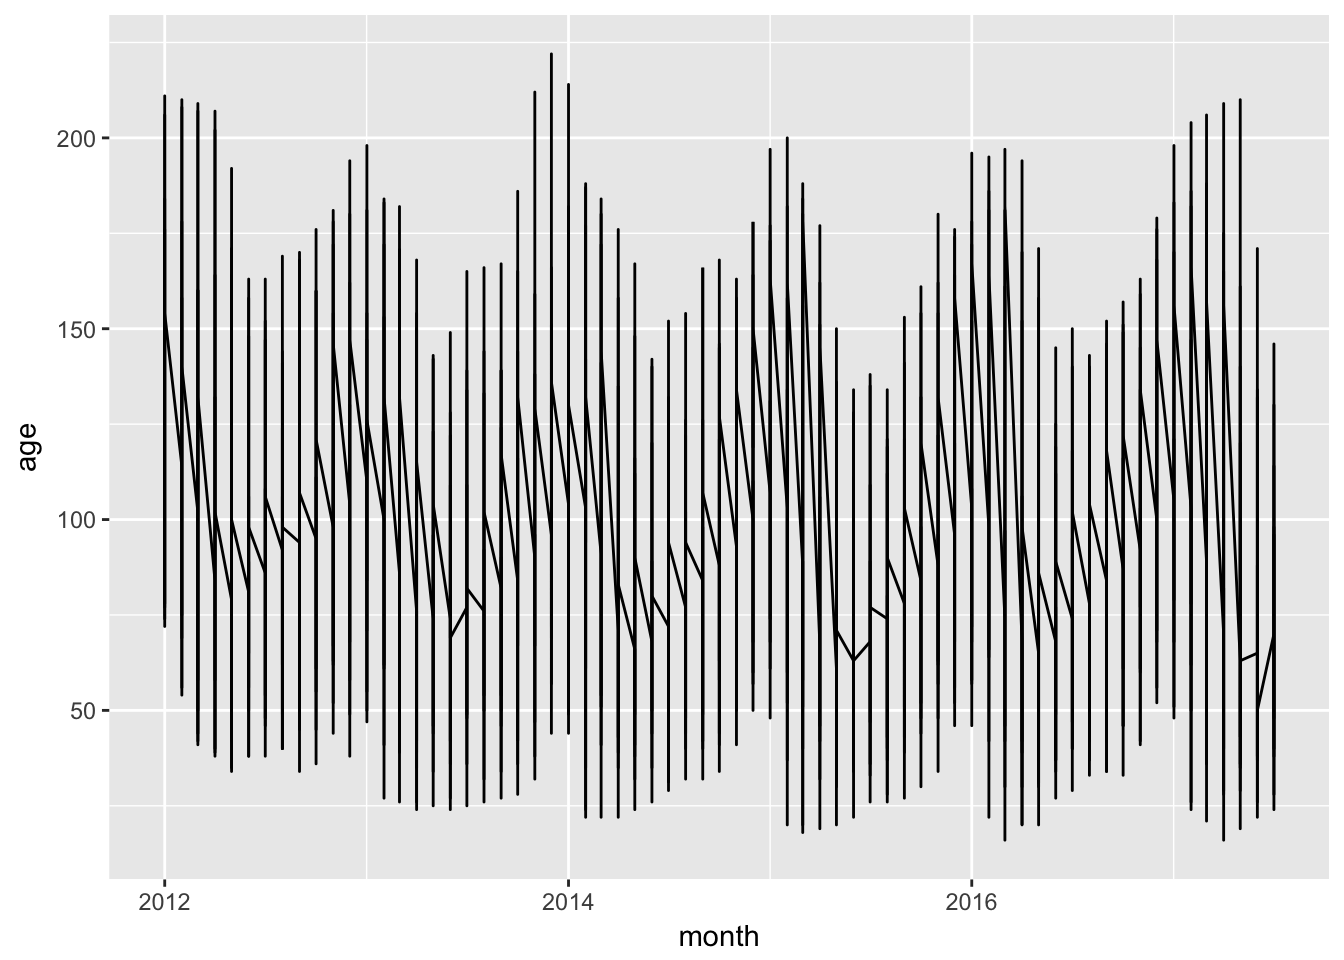
\includegraphics{jonpage-r-course_files/figure-latex/unnamed-chunk-4-1.pdf}

Scatterplot of two dimensions

\begin{verbatim}
plot(swiss[,c("Education", "Fertility")])
# or
plot(swiss[4,1])
# or
plot(swiss$Education, swiss$Fertility)
# or
plot(swiss$Fertility ~ swiss$Education)
\end{verbatim}

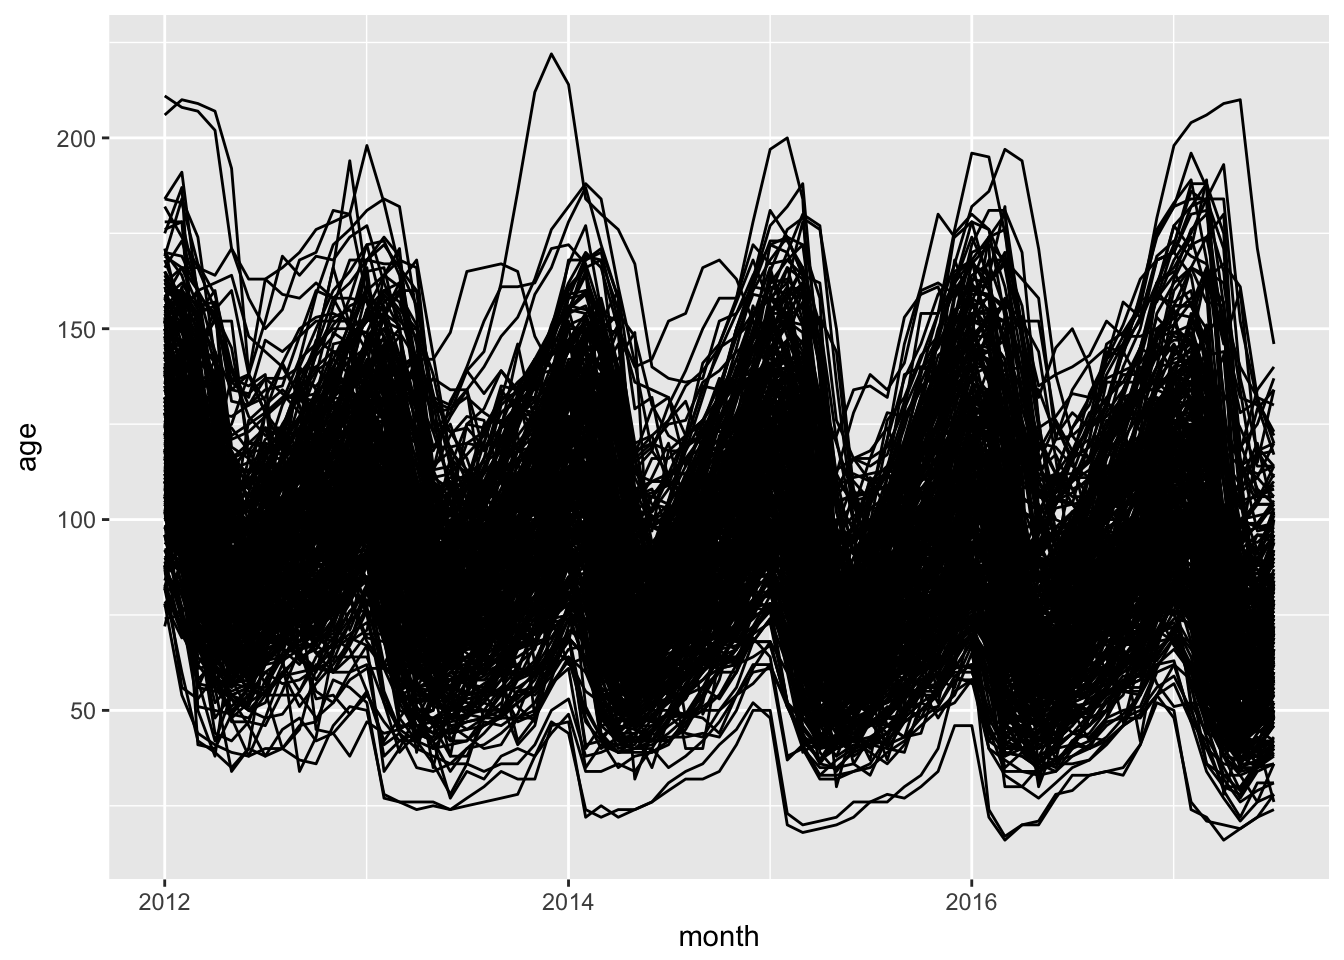
\includegraphics{jonpage-r-course_files/figure-latex/unnamed-chunk-5-1.pdf}

Smoothed Scatterplot of two dimensions

\begin{Shaded}
\begin{Highlighting}[]
\KeywordTok{smoothScatter}\NormalTok{(swiss$Fertility ~}\StringTok{ }\NormalTok{swiss$Examination)}
\end{Highlighting}
\end{Shaded}

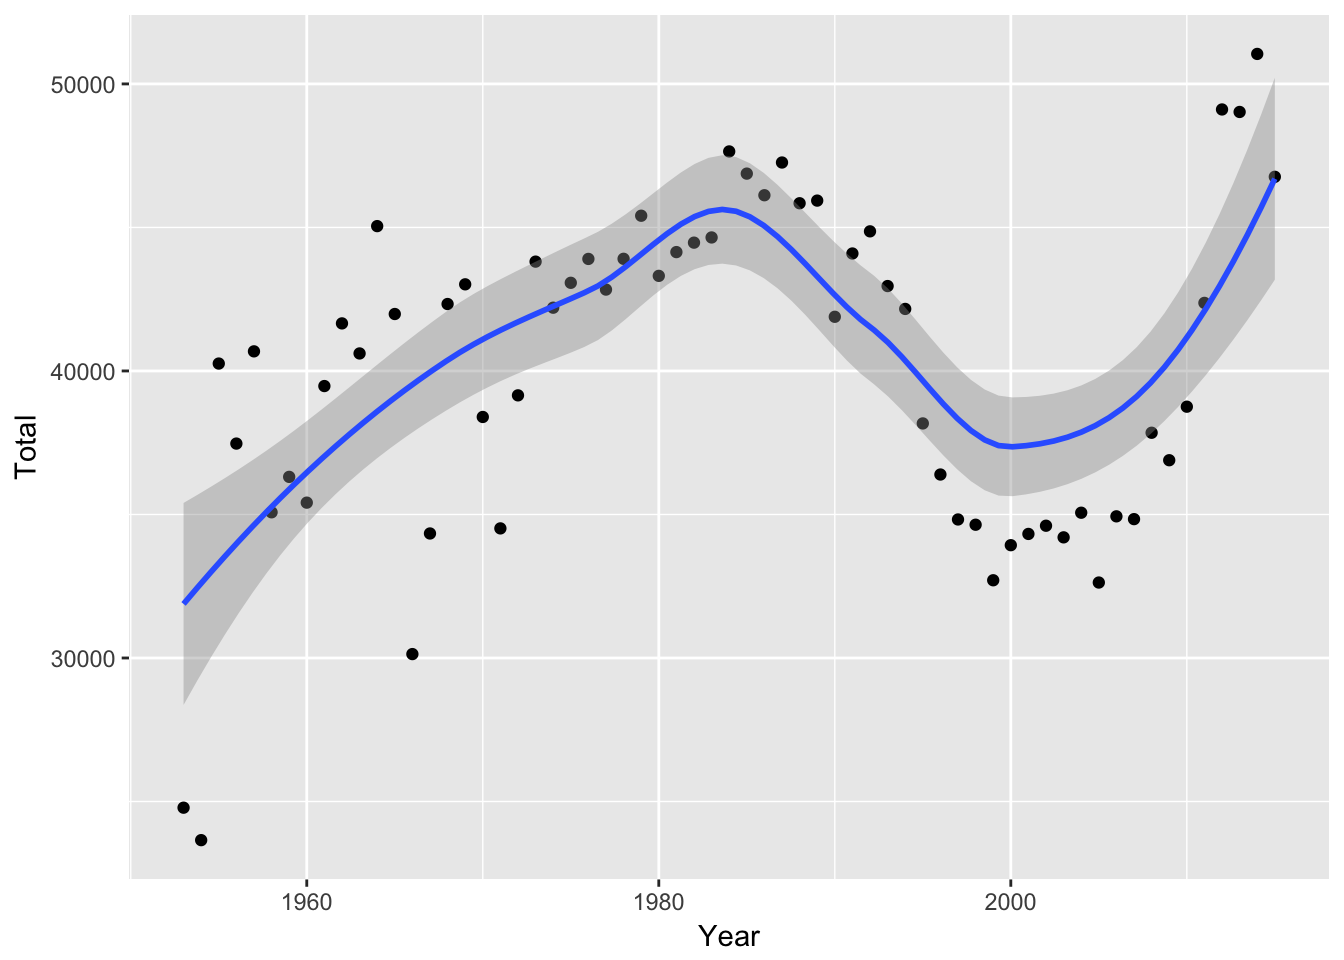
\includegraphics{jonpage-r-course_files/figure-latex/unnamed-chunk-6-1.pdf}

Scatterplot with a \texttt{loess} (locally weighted polynomial
regression)

\begin{Shaded}
\begin{Highlighting}[]
\KeywordTok{smoothScatter}\NormalTok{(swiss$Fertility ~}\StringTok{ }\NormalTok{swiss$Agriculture)}
\end{Highlighting}
\end{Shaded}

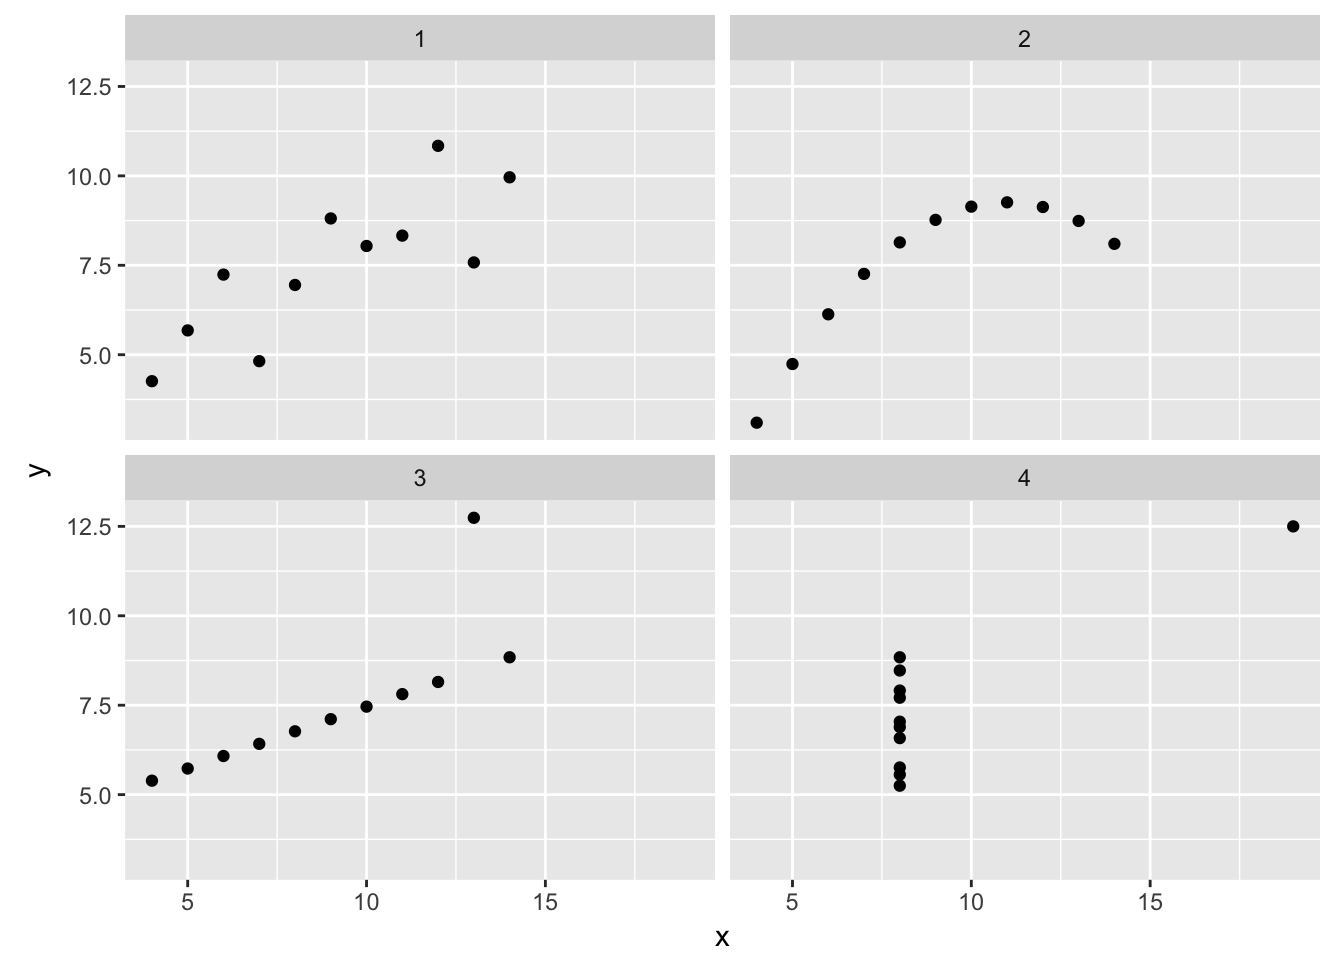
\includegraphics{jonpage-r-course_files/figure-latex/unnamed-chunk-7-1.pdf}

\subsection{Distribution plots}\label{distribution-plots}

Histograms:

\begin{Shaded}
\begin{Highlighting}[]
\KeywordTok{hist}\NormalTok{(swiss$Catholic)}
\end{Highlighting}
\end{Shaded}

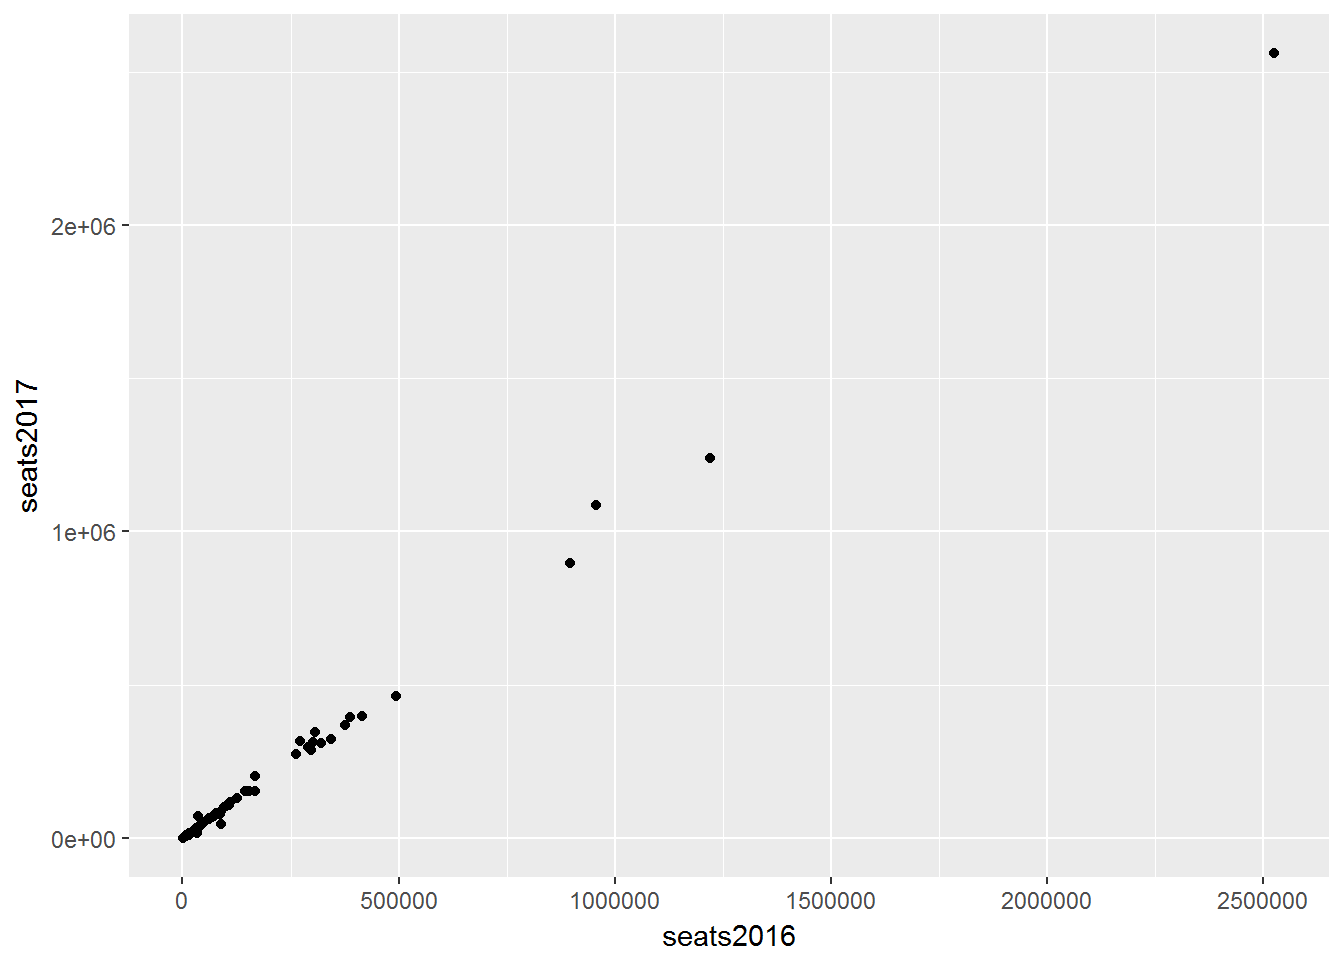
\includegraphics{jonpage-r-course_files/figure-latex/unnamed-chunk-8-1.pdf}

Stem-and-Leaf Plots:

\begin{Shaded}
\begin{Highlighting}[]
\KeywordTok{stem}\NormalTok{(swiss$Fertility)}
\end{Highlighting}
\end{Shaded}

\begin{verbatim}
## 
##   The decimal point is 1 digit(s) to the right of the |
## 
##   3 | 5
##   4 | 35
##   5 | 46778
##   6 | 124455556678899
##   7 | 01223346677899
##   8 | 0233467
##   9 | 223
\end{verbatim}

Kernel density plot (and add a rug showing where observation occur):

\begin{Shaded}
\begin{Highlighting}[]
\KeywordTok{plot}\NormalTok{(}\KeywordTok{density}\NormalTok{(swiss$Fertility))}
\KeywordTok{rug}\NormalTok{(swiss$Fertility)}
\end{Highlighting}
\end{Shaded}

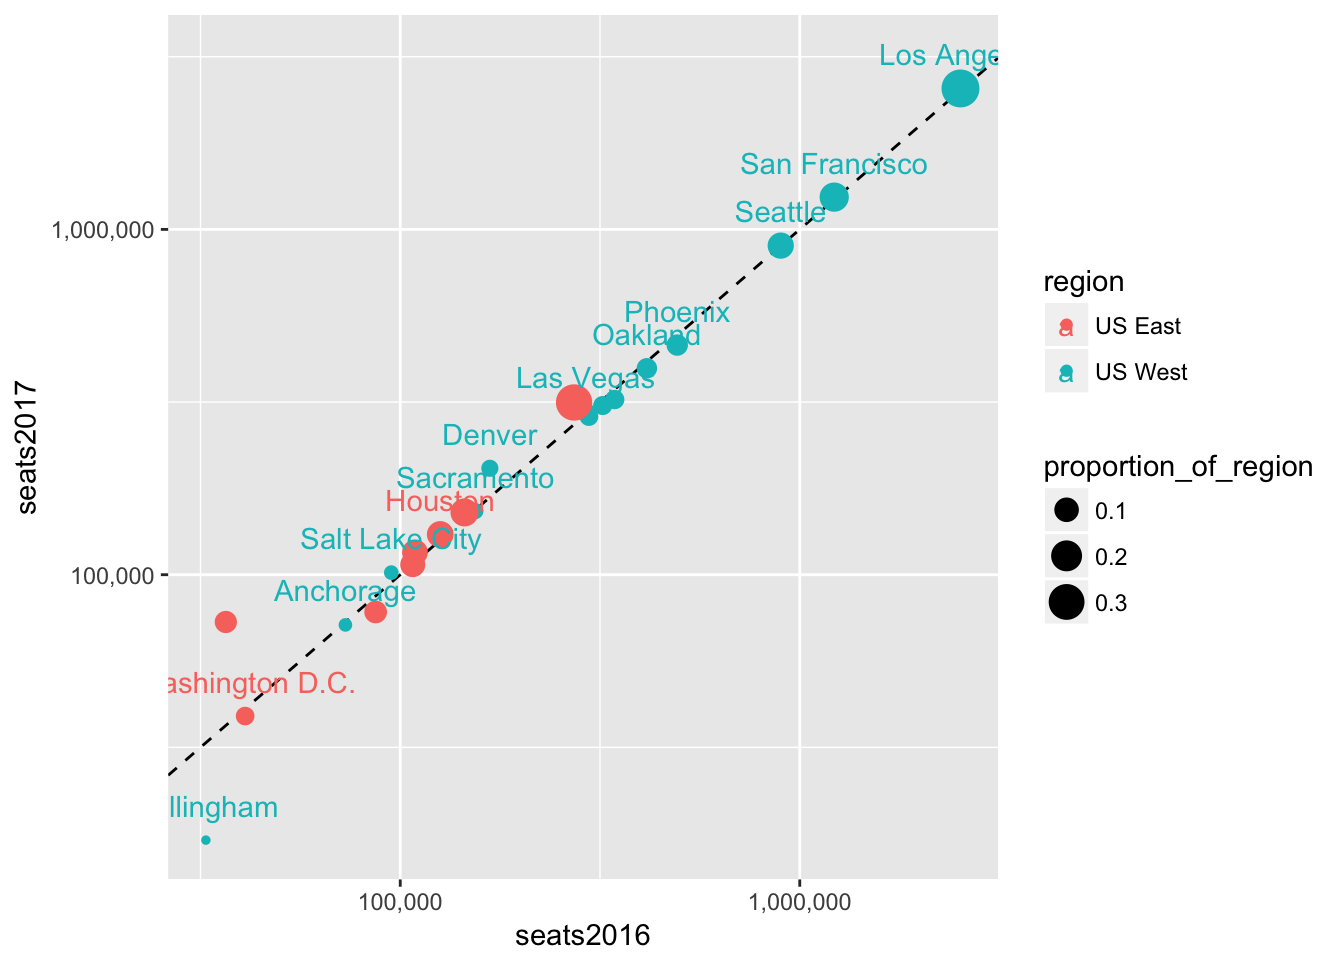
\includegraphics{jonpage-r-course_files/figure-latex/unnamed-chunk-10-1.pdf}

Boxplots:

\begin{Shaded}
\begin{Highlighting}[]
\KeywordTok{boxplot}\NormalTok{(swiss)}
\end{Highlighting}
\end{Shaded}

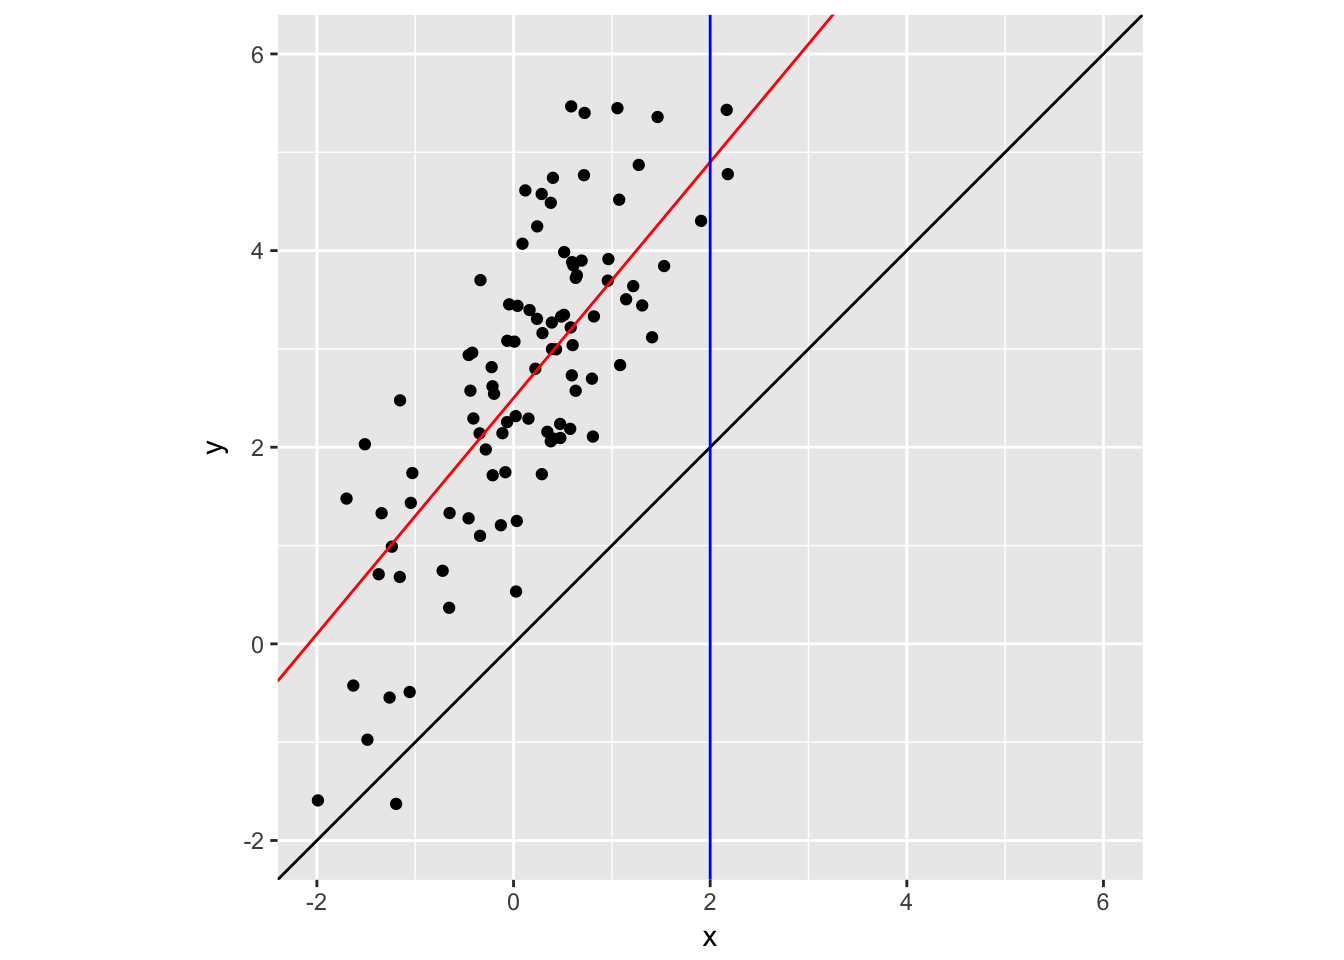
\includegraphics{jonpage-r-course_files/figure-latex/unnamed-chunk-11-1.pdf}

\subsubsection{More complicated charts}\label{more-complicated-charts}

Conditioning plots:

\begin{Shaded}
\begin{Highlighting}[]
\KeywordTok{coplot}\NormalTok{(swiss$Fertility ~}\StringTok{ }\NormalTok{swiss$Examination |}\StringTok{ }\KeywordTok{as.factor}\NormalTok{(swiss$Catholic >}\StringTok{ }\DecValTok{50}\NormalTok{))}
\end{Highlighting}
\end{Shaded}

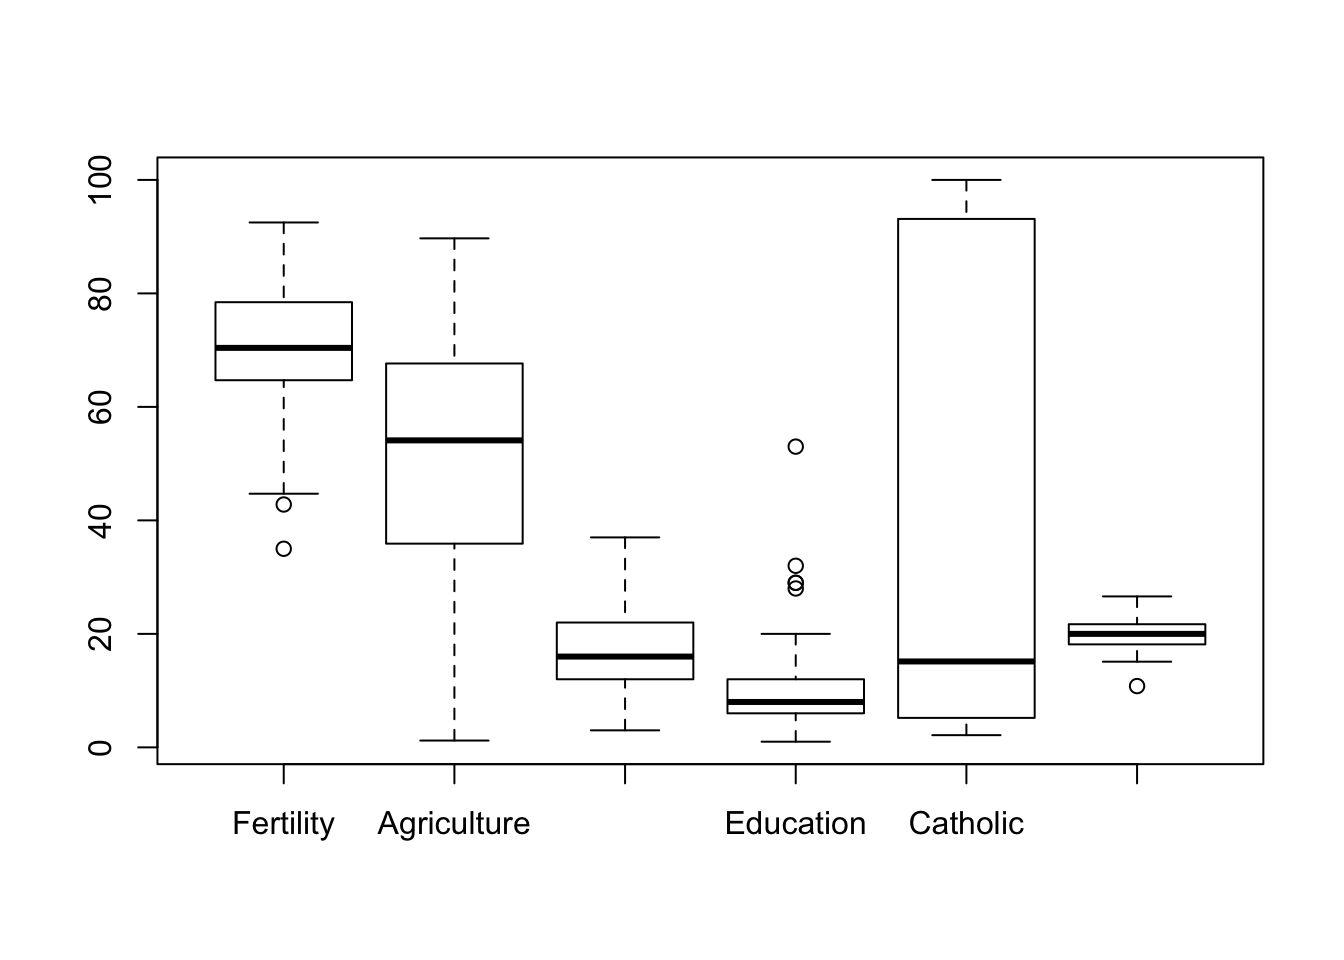
\includegraphics{jonpage-r-course_files/figure-latex/unnamed-chunk-12-1.pdf}

Star plots (half-star plots here):

\begin{Shaded}
\begin{Highlighting}[]
\KeywordTok{stars}\NormalTok{(swiss, }\DataTypeTok{key.loc =} \KeywordTok{c}\NormalTok{(}\DecValTok{15}\NormalTok{,}\DecValTok{1}\NormalTok{), }\DataTypeTok{flip.labels =} \OtherTok{FALSE}\NormalTok{, }\DataTypeTok{full =} \OtherTok{FALSE}\NormalTok{)}
\end{Highlighting}
\end{Shaded}

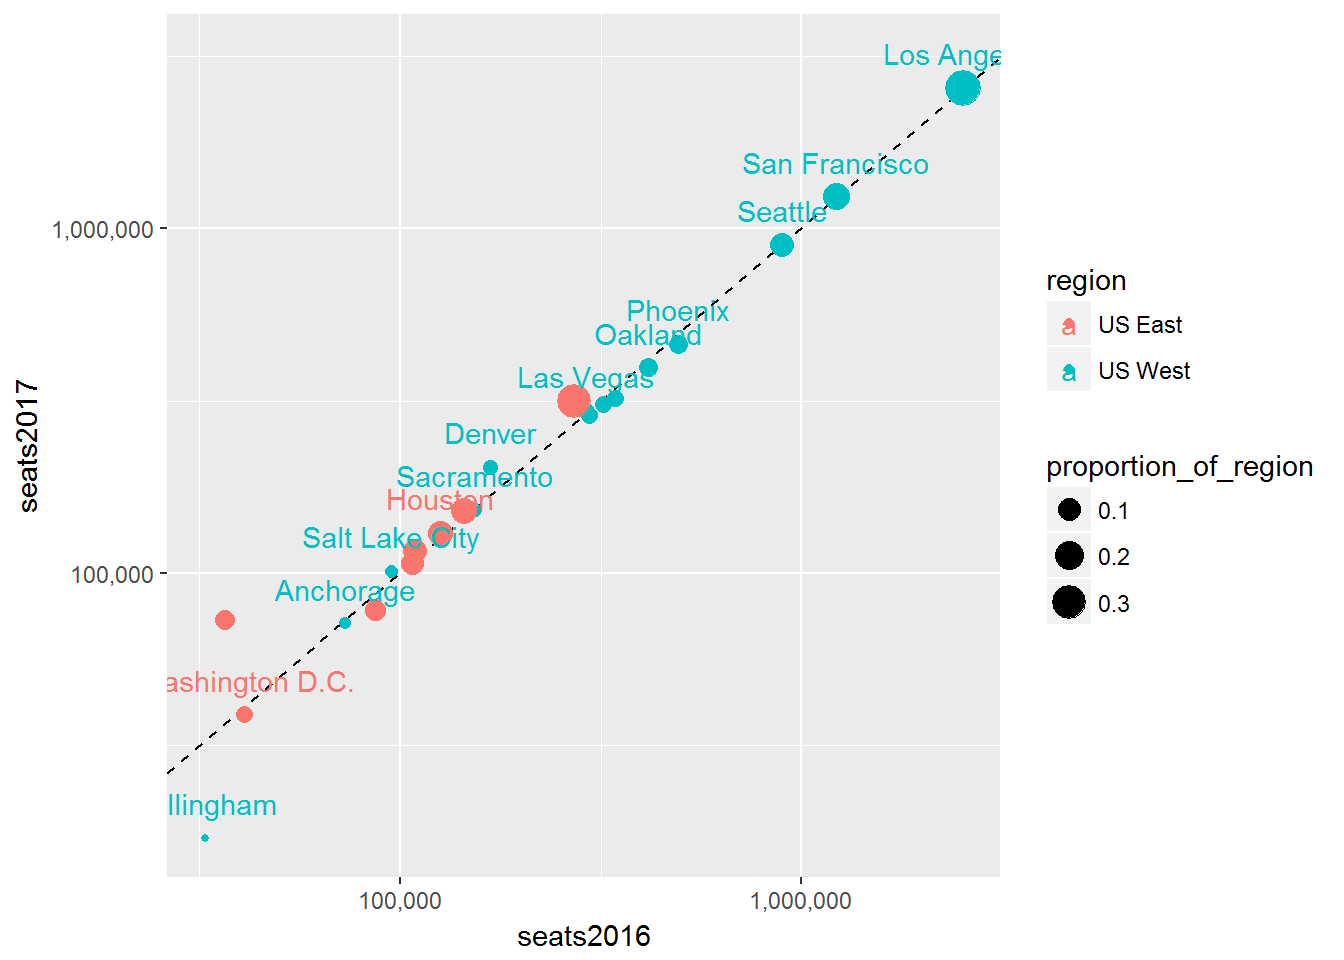
\includegraphics{jonpage-r-course_files/figure-latex/unnamed-chunk-13-1.pdf}

\section{Assignment}\label{assignment}

Choose a dataset from \texttt{datasets}
(\texttt{library(help\ =\ "datasets")} will show you a list) and create
5 charts in an R Markdown file from the example charts above. Run the
following command to see what else is available in the base R graphics
package:

\begin{verbatim}
demo(graphics)
\end{verbatim}

\chapter{Literature}\label{literature}

Here is a review of existing methods.

\chapter{Methods}\label{methods}

We describe our methods in this chapter.

\chapter{Applications}\label{applications}

Some \emph{significant} applications are demonstrated in this chapter.

\section{Example one}\label{example-one}

\section{Example two}\label{example-two}

\chapter{Final Words}\label{final-words}

We have finished a nice book.

\hypertarget{trifecta}{\chapter{How to Judge
Visualizations}\label{trifecta}}

\section{Pre-class assignment}\label{pre-class-assignment}

Read
\href{http://junkcharts.typepad.com/junk_charts/junk-charts-trifecta-checkup-the-definitive-guide.html}{Junk
Charts Trifecta Checkup}

\section{Lecture}\label{lecture}

\href{http://junkcharts.typepad.com/numbersruleyourworld/biography.html}{Kaiser
Fung} has a useful framework for judging the quality of data
visualizations. He calls his framework the
\href{http://junkcharts.typepad.com/junk_charts/junk-charts-trifecta-checkup-the-definitive-guide.html}{Junk
Charts Trifecta Checkup}. To make that shorter, we'll just call this
framework the \emph{Trifecta Checkup}. This framework boils down to the
following 3 questions:

\begin{enumerate}
\def\labelenumi{\arabic{enumi}.}
\tightlist
\item
  What is the \textbf{question}?
\item
  What does the \textbf{data} say?
\item
  What does the \textbf{visual} say?
\end{enumerate}

Each visualization can be labeled according to which question(s) it does
not answer well. For example, a chart with a meaningful question and
relevant data, but ineffective visuals, would be labeled \textbf{v}. A
chart that gets the data and question wrong, but has a nice visual,
would be labeled \textbf{qd}.

\section{Assignment}\label{assignment-1}

Assign a label to each of the following visualizations based on the
\emph{Trifecta Checkup}. Provide at least one sentence per question
defending your chosen labels.

\bibliography{packages,book}


\end{document}
